\chapter{Unsur-Unsur di Alam Semesta dan di Bumi}\label{ch:g9:elements-universe-earth}

Kalsium di tulangmu, besi di darahmu, dan oksigen yang kamu hirup tidak
dibuat di Bumi. Semuanya dibuat di dalam bintang-bintang yang hidup dan
mati sebelum Matahari lahir, dan semuanya telah berpindah dari batuan ke
laut, dari laut ke tumbuhan, dari tumbuhan ke hewan, selama miliaran
tahun. Ada unsur yang terdapat di mana-mana, ada yang langka. Unsur-unsur
apa yang menyusun bintang, Bumi, samudra --- dan kita?

\begin{recall}
\omterm{def:g9:inside-the-atom:element}{Unsur kimia} adalah himpunan \omterm{def:g7:atoms-and-molecules:atom}{atom} dengan \omterm{def:g9:inside-the-atom:atomic-number}{nomor atom} $Z$ yang sama; massa
sebuah \omterm{def:g7:atoms-and-molecules:atom}{atom} mendekati $A \times \qty{1.67e-27}{kg}$, dengan $A$ \omterm{def:g9:inside-the-atom:atomic-number}{nomor
massanya} (\cref{ch:g9:inside-the-atom}). \omterm{def:g9:periodic-table-first-look:periodic-table}{Tabel periodik} mendaftar 118
unsur menurut \omterm{def:g9:inside-the-atom:atomic-number}{nomor atomnya} (\cref{ch:g9:periodic-table-first-look}).
\omterm{def:g4:air-a-mixture-of-gases:air}{Udara} terdiri atas sekitar empat perlima nitrogen dan seperlima oksigen
(\cref{ch:g4:air-a-mixture-of-gases}).
\end{recall}

\section{Unsur-unsur bintang}

\begin{definition}[Kelimpahan]\label{def:g9:elements-universe-earth:abundance}
Yang disebut \emph{kelimpahan}\index{kelimpahan} sebuah unsur dalam
sebuah benda materi --- bintang, kerak Bumi, samudra, makhluk hidup ---
adalah bagiannya dari massa total, biasanya dinyatakan dalam persen.
\end{definition}

\begin{proposition}[Matahari adalah hidrogen dan helium]\label{prop:g9:elements-universe-earth:sun}
% ledger: ab:sun-X, ab:sun-Y, ab:sun-Z
Permukaan Matahari terdiri atas, menurut massa, sekitar
\qty{74}{\percent} hidrogen dan \qty{25}{\percent} helium; semua unsur
lainnya bersama-sama hanya sekitar \qty{1.3}{\percent}. Sebagian besar
materi alam semesta yang terlihat memiliki susunan serupa: hidrogen dan
helium, dengan sejumput segala yang lain.
\end{proposition}

\begin{proposition}[Unsur-unsur yang dibuat di dalam bintang]\label{prop:g9:elements-universe-earth:stars}
Hidrogen dan sebagian besar helium terbentuk pada menit-menit pertama
alam semesta. Hampir semua unsur yang lebih berat --- karbon, oksigen,
besi, emas --- dibuat kemudian, di dalam bintang, dan tersebar ke
antariksa ketika bintang-bintang meledak. Bintang dan planet baru
terbentuk dari debu yang diperkaya itu. Cara bintang melakukannya
diceritakan di buku fisika.
\end{proposition}

\begin{omfigure}
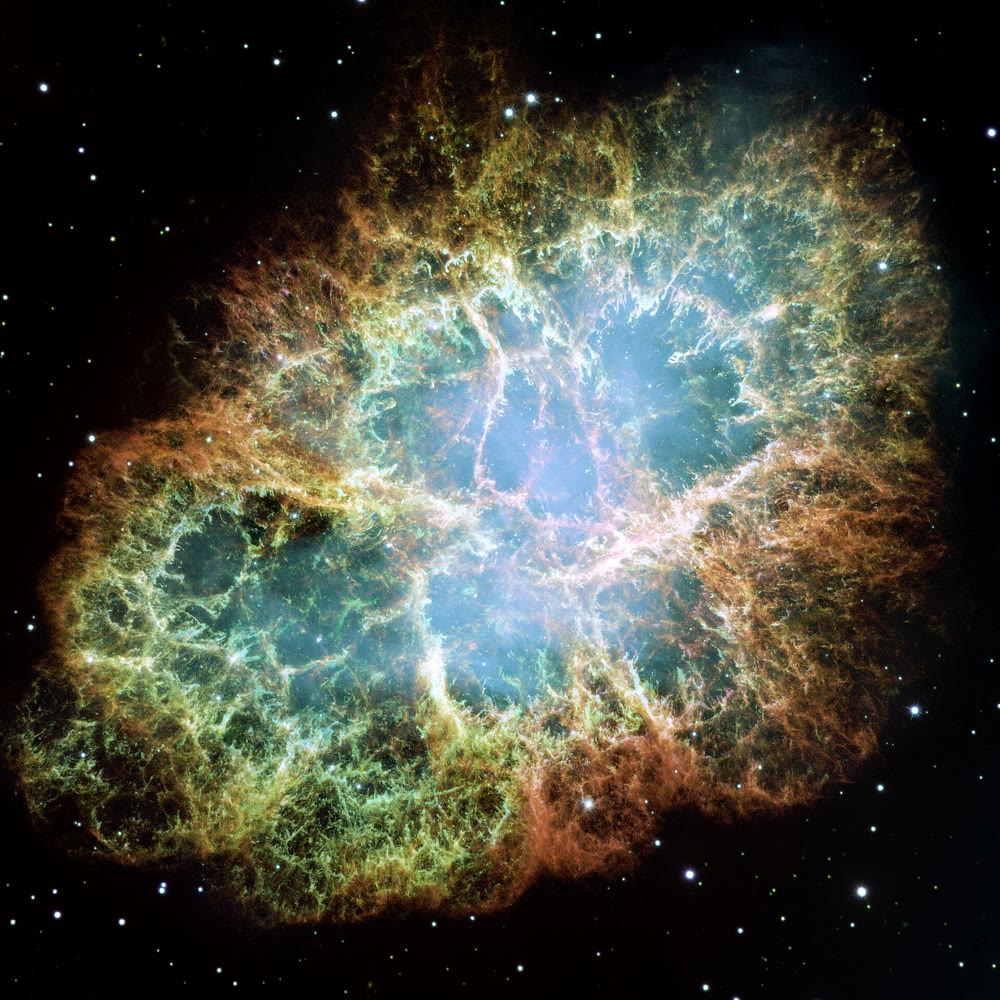
\includegraphics[width=0.45\linewidth]{images/book1/crab-nebula.jpg}

{\small Nebula Kepiting, awan yang ditinggalkan sebuah bintang yang
meledak hampir seribu tahun yang lalu, yang menyebarkan unsur-unsur baru
ke antariksa (NASA, ESA, J.~Hester dan A.~Loll).}
\end{omfigure}

\section{Bumi}

\begin{proposition}[Kerak Bumi]\label{prop:g9:elements-universe-earth:crust}
% ledger: ab:crust-O, ab:crust-Si, ab:crust-Al, ab:crust-Fe, ab:crust-Ca, ab:crust-Na, ab:crust-K, ab:crust-Mg, ab:crust-first10
Kulit Bumi yang tipis dan berbatu, yaitu kerak, terdiri atas hampir
separuh oksigen dan lebih dari seperempat silikon menurut massa: batuan
dan pasir sebagian besar berupa oksida silikon dan oksida beberapa
\omterm{def:g9:periodic-table-first-look:metal}{logam}. Delapan unsur --- oksigen, silikon, aluminium, besi, kalsium,
natrium, kalium, magnesium --- menyusun sekitar \qty{99}{\percent}
kerak itu. Hidrogen dan helium, yang begitu umum di bintang-bintang,
langka di sini: gas-gas ringan itu lolos dari Bumi muda.
\end{proposition}

\begin{remark}[Di dalam Bumi]\label{rem:g9:elements-universe-earth:core}
Kerak bukan seluruh Bumi. Besi, yang berat, tenggelam ke arah pusat
ketika Bumi muda masih cair: inti Bumi sebagian besar berupa besi,
dengan sedikit nikel.
\end{remark}

\begin{proposition}[Samudra dan udara]\label{prop:g9:elements-universe-earth:ocean}
% ledger: sea:salts-share, sea:NaCl-ions, sea:MgSO4-ions, air:N2, air:O2
Air laut sebagian besar berupa air --- hidrogen dan oksigen --- dengan
sekitar \qty{3.5}{\percent} garam-garam terlarut menurut massa. Di antara
\omterm{def:g9:ions:ion}{ion-ion} terlarut, klorida dan natrium menyusun sekitar
\qty{85}{\percent}, magnesium dan sulfat \qty{10}{\percent} lagi. \omterm{def:g4:air-a-mixture-of-gases:air}{Udara}
sebagian besar berupa nitrogen dan oksigen.
\end{proposition}

\begin{omfigure}
\begin{tikzpicture}
\begin{axis}[xbar, width=0.40\linewidth, height=5.4cm, xmin=0, xmax=85,
    bar width=7pt, symbolic y coords={Mg,K,Na,Ca,Fe,Al,Si,O}, ytick=data,
    xlabel={persen massa}, title={\small kerak Bumi},
    nodes near coords, nodes near coords style={font=\scriptsize},
    tick label style={font=\small}, label style={font=\small},
    axis lines*=left, enlarge y limits=0.08]
% ledger: ab:crust-O, ab:crust-Si, ab:crust-Al, ab:crust-Fe, ab:crust-Ca, ab:crust-Na, ab:crust-K, ab:crust-Mg
\addplot[fill=omDef!45, draw=omDef] coordinates {(46.6,O) (27.7,Si) (8.1,Al)
  (5.0,Fe) (3.6,Ca) (2.8,Na) (2.6,K) (2.1,Mg)};
\end{axis}
\end{tikzpicture}\hfill
\begin{tikzpicture}
\begin{axis}[xbar, width=0.40\linewidth, height=5.4cm, xmin=0, xmax=85,
    bar width=7pt, symbolic y coords={{P},{N},{Ca},{H},{C},{O}}, ytick=data,
    xlabel={persen massa}, title={\small tubuh manusia},
    nodes near coords, nodes near coords style={font=\scriptsize},
    tick label style={font=\small}, label style={font=\small},
    axis lines*=left, enlarge y limits=0.1]
% ledger: body:atoms-O, body:atoms-C, body:atoms-H, body:atoms-N, body:atoms-Ca, body:atoms-P (masses = atoms x atomic mass, over 70 kg)
\addplot[fill=omProp!45, draw=omProp] coordinates {(61.1,O) (22.9,C) (10.1,H)
  (1.3,N) (1.5,Ca) (0.7,P)};
\end{axis}
\end{tikzpicture}

{\small \omterm{def:g9:elements-universe-earth:abundance}{Kelimpahan} menurut massa. Kiri: delapan unsur utama kerak Bumi.
Kanan: enam unsur utama tubuh manusia dewasa yang ramping (dihitung dari
perkiraan banyaknya \omterm{def:g7:atoms-and-molecules:atom}{atom}).}
\end{omfigure}

\section{Tubuh manusia}

\begin{proposition}[Dari apa kita tersusun]\label{prop:g9:elements-universe-earth:body}
% ledger: body:atoms-O, body:atoms-C, body:atoms-H, body:atoms-N, body:atoms-Ca, body:atoms-P, body:atoms-total
Menurut massa, tubuh orang dewasa yang ramping terdiri atas sekitar
\qty{61}{\percent} oksigen, \qty{23}{\percent} karbon, dan
\qty{10}{\percent} hidrogen --- sebagian besar di dalam air dan di dalam
\omterm{def:g7:atoms-and-molecules:molecule}{molekul-molekul} kehidupan --- diikuti nitrogen, kalsium (di tulang dan
gigi), dan fosfor. Jika dihitung menurut banyaknya \omterm{def:g7:atoms-and-molecules:atom}{atom} alih-alih massa,
urutannya berubah: \omterm{def:g7:atoms-and-molecules:atom}{atom} hidrogen di dalam tubuh lebih banyak daripada
semua \omterm{def:g7:atoms-and-molecules:atom}{atom} lainnya bersama-sama, karena \omterm{def:g7:atoms-and-molecules:atom}{atom} hidrogen begitu ringan.
Tubuh seberat \qty{70}{kg} mengandung sekitar $7 \times 10^{27}$ \omterm{def:g7:atoms-and-molecules:atom}{atom}.
\end{proposition}

\begin{method}[Membaca diagram kelimpahan]\label{met:g9:elements-universe-earth:read}
\begin{enumerate}
  \item Periksalah apa yang diukur: massa (pada kebanyakan diagram) atau
        banyaknya \omterm{def:g7:atoms-and-molecules:atom}{atom}.
  \item Bacalah bagian setiap unsur; jumlahkan bagian unsur-unsur utama
        untuk melihat seberapa banyak yang dicakupnya.
  \item Untuk membandingkan dua benda, carilah unsur-unsur yang sama-sama
        ada pada keduanya dan unsur-unsur yang hanya ada pada salah satunya.
\end{enumerate}
Oksigen berada di puncak kedua diagram dalam bab ini: oksigen adalah
unsur yang paling umum di kerak Bumi dan di tubuh manusia menurut massa.
\end{method}

\section{Atom-atom yang sama, didaur ulang}

\begin{example}[Perjalanan sebuah atom karbon]\label{ex:g9:elements-universe-earth:journey}
Sebuah \omterm{def:g7:atoms-and-molecules:atom}{atom} karbon yang dibuat di dalam bintang lama berselang dapat
berdiam selama jutaan tahun di dalam batu kapur, dilepaskan sebagai
karbon dioksida oleh gunung berapi, diambil oleh sehelai daun, menjadi
bagian dari gula di dalam buah, berpindah ke hewan yang memakan buah
itu, lalu diembuskan lagi sebagai karbon dioksida. \omterm{def:g7:atoms-and-molecules:atom}{Atom} tidak dimusnahkan
oleh \omterm{def:g5:irreversible-changes:chemical-change}{perubahan kimia}: \omterm{def:g7:atoms-and-molecules:atom}{atom} diteruskan.
\end{example}

\begin{omfigure}
\begin{tikzpicture}[font=\small,
    box/.style={draw=omDef, fill=omDef!6, rounded corners=2pt, align=center,
      minimum height=0.85cm, text width=2.3cm}]
  \node[box] (a) at (0,2.2) {di dalam batuan\\ (batu kapur)};
  \node[box] (b) at (4.3,2.2) {di udara\\ (\ce{CO2})};
  \node[box] (c) at (8.6,2.2) {di dalam daun\\ (gula)};
  \node[box] (d) at (8.6,0) {di dalam hewan};
  \node[box] (e) at (4.3,0) {diembuskan\\ (\ce{CO2})};
  \draw[->, thick, omProp] (a) -- node[above, font=\footnotesize] {gunung api} (b);
  \draw[->, thick, omProp] (b) -- (c);
  \draw[->, thick, omProp] (c) -- node[right, font=\footnotesize] {dimakan} (d);
  \draw[->, thick, omProp] (d) -- (e);
  \draw[->, thick, omProp] (e) -- (b);
\end{tikzpicture}

{\small Sebuah \omterm{def:g7:atoms-and-molecules:atom}{atom} karbon berpindah dari batuan ke \omterm{def:g4:air-a-mixture-of-gases:air}{udara} ke daun ke
hewan lalu kembali ke \omterm{def:g4:air-a-mixture-of-gases:air}{udara}: \omterm{def:g7:atoms-and-molecules:atom}{atom} itu sendiri tidak pernah dimusnahkan.}
\end{omfigure}

\begin{omfigure}
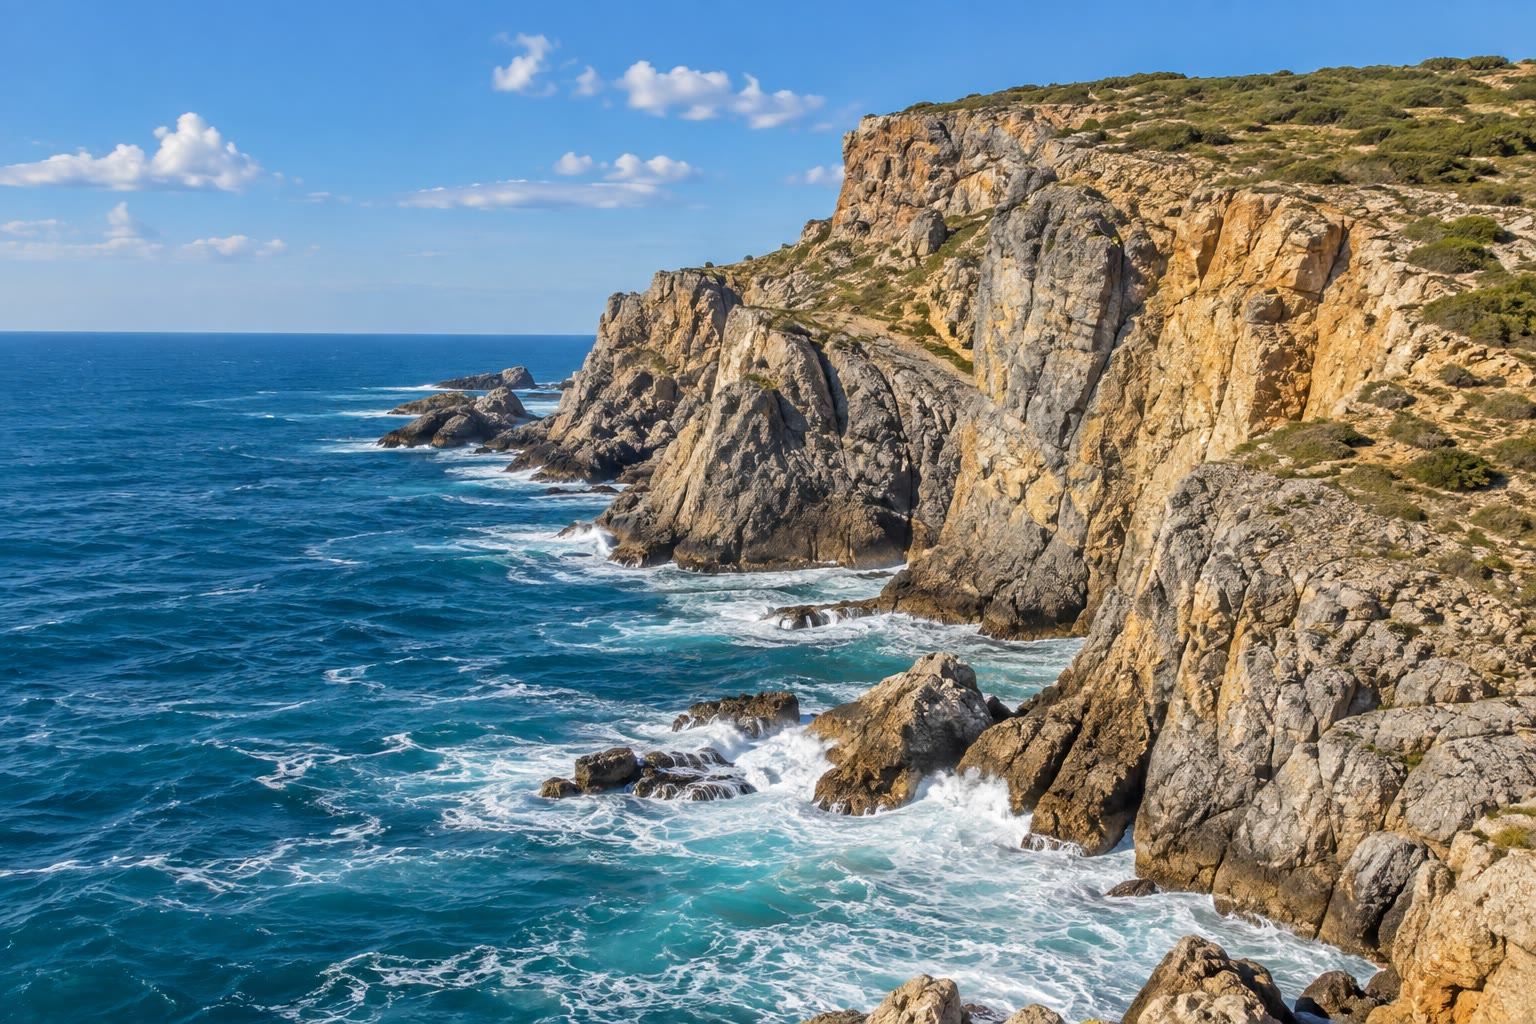
\includegraphics[width=0.55\linewidth]{images/book1/ai/g9-coastal-cliff.jpg}

{\small Batuan, laut, dan \omterm{def:g4:air-a-mixture-of-gases:air}{udara}: tiga \omterm{def:g6:pure-substances-and-mixtures:mixture}{campuran} yang sangat berbeda dari
unsur-unsur yang sama.}
\end{omfigure}

\section{Latihan}

\begin{exercise}[$\star$]\label{exo:g9:elements-universe-earth:1}
Dua unsur apa yang menyusun hampir seluruh Matahari?
\end{exercise}

\begin{exercise}[$\star$]\label{exo:g9:elements-universe-earth:2}
Unsur apa yang paling melimpah di kerak Bumi? Di tubuh manusia (menurut
massa)?
\end{exercise}

\begin{exercise}[$\star$]\label{exo:g9:elements-universe-earth:3}
Di mana sebagian besar unsur yang lebih berat daripada helium dibuat?
\end{exercise}

\begin{exercise}[$\star$]\label{exo:g9:elements-universe-earth:4}
Berapa persen massa air laut yang berupa garam terlarut?
\end{exercise}

\begin{exercise}[$\star\star$]\label{exo:g9:elements-universe-earth:5}
Dengan diagram kerak Bumi, jumlahkan bagian oksigen dan silikon.
Kira-kira berapa bagian kerak Bumi itu?
\end{exercise}

\begin{exercise}[$\star\star$]\label{exo:g9:elements-universe-earth:6}
Mengapa hidrogen dan helium begitu sedikit di kerak Bumi, padahal
Matahari hampir seluruhnya tersusun atas keduanya?
\end{exercise}

\begin{exercise}[$\star\star$]\label{exo:g9:elements-universe-earth:7}
Berapa massa karbon dalam tubuh seberat \qty{70}{kg} yang mengandung
\qty{23}{\percent} karbon?
\end{exercise}

\begin{exercise}[$\star\star$]\label{exo:g9:elements-universe-earth:8}
Mengapa oksigen merupakan unsur yang paling umum di dalam tubuh menurut
massa, sedangkan hidrogen yang paling umum menurut banyaknya \omterm{def:g7:atoms-and-molecules:atom}{atom}?
\end{exercise}

\begin{exercise}[$\star\star$]\label{exo:g9:elements-universe-earth:9}
Sebongkah granit \qty{1000}{kg} adalah potongan kerak yang khas. Dengan
diagram itu, kira-kira berapa massa aluminium yang dikandungnya?
\end{exercise}

\begin{exercise}[$\star\star$]\label{exo:g9:elements-universe-earth:10}
Unsur-unsur apa yang muncul di antara unsur-unsur utama kerak Bumi
maupun tubuh manusia?
\end{exercise}

\begin{exercise}[$\star\star\star$]\label{exo:g9:elements-universe-earth:11}
Tubuh seberat \qty{70}{kg} mengandung sekitar \qty{1.06}{kg} kalsium.
Hitung massa satu \omterm{def:g7:atoms-and-molecules:atom}{atom} kalsium ($A = 40$), lalu banyaknya \omterm{def:g7:atoms-and-molecules:atom}{atom} kalsium.
Tuliskan dalam notasi ilmiah.
\end{exercise}

\begin{exercise}[$\star\star\star$]\label{exo:g9:elements-universe-earth:12}
\omterm{def:g7:atoms-and-molecules:atom}{Atom-atom} tubuhmu semuanya pernah menjadi bagian dari benda lain.
Pakailah perjalanan sebuah \omterm{def:g7:atoms-and-molecules:atom}{atom} karbon untuk menjelaskan mengapa jumlah
total \omterm{def:g7:atoms-and-molecules:atom}{atom} karbon di Bumi hampir tidak berubah.
\end{exercise}

\section{Soal: Berapa Atomkah Aku?}

\begin{problem}[{Soal akhir pekan --- dari diagram kelimpahan sampai
banyaknya atom oksigen dalam tubuh manusia}]
\label{pb:g9:elements-universe-earth:1}
% ledger: body:atoms-O, body:atoms-total
Seorang dewasa yang ramping seberat \qty{70}{kg} terdiri atas, menurut
massa, sekitar \qty{61}{\percent} oksigen, \qty{23}{\percent} karbon,
dan \qty{10}{\percent} hidrogen. Anggaplah massa sebuah \omterm{def:g9:inside-the-atom:proton}{nukleon}
\qty{1.67e-27}{kg}; sebuah \omterm{def:g7:atoms-and-molecules:atom}{atom} oksigen memiliki 16 \omterm{def:g9:inside-the-atom:proton}{nukleon}, \omterm{def:g7:atoms-and-molecules:atom}{atom} karbon
12, \omterm{def:g7:atoms-and-molecules:atom}{atom} hidrogen 1. \omterm{def:g9:inside-the-atom:nucleus}{Elektron} diabaikan.

\medskip
\noindent\textbf{Bagian I --- Massanya.}
\begin{enumerate}
  \item Hitung massa oksigen di dalam tubuh.
  \item Hitung massa karbon dan massa hidrogen.
  \item Berapa persen massa yang disusun ketiga unsur ini bersama-sama?
  \item Sebagian besar oksigen dan hidrogen ini berada dalam satu
        senyawa. Senyawa apa?
\end{enumerate}

\medskip
\noindent\textbf{Bagian II --- Satu \omterm{def:g7:atoms-and-molecules:atom}{atom}.}
\begin{enumerate}[resume]
  \item Hitung massa satu \omterm{def:g7:atoms-and-molecules:atom}{atom} oksigen.
  \item Hitung massa satu \omterm{def:g7:atoms-and-molecules:atom}{atom} karbon dan satu \omterm{def:g7:atoms-and-molecules:atom}{atom} hidrogen.
  \item Berapa \omterm{def:g7:atoms-and-molecules:atom}{atom} hidrogen yang beratnya sama dengan satu \omterm{def:g7:atoms-and-molecules:atom}{atom} oksigen?
  \item Mengapa \omterm{def:g9:inside-the-atom:nucleus}{elektron} dapat diabaikan?
\end{enumerate}

\medskip
\noindent\textbf{Bagian III --- Hitungannya.}
\begin{enumerate}[resume]
  \item Hitung banyaknya \omterm{def:g7:atoms-and-molecules:atom}{atom} hidrogen di dalam tubuh.
  \item Hitung banyaknya \omterm{def:g7:atoms-and-molecules:atom}{atom} karbon.
  \item Hitung banyaknya \omterm{def:g7:atoms-and-molecules:atom}{atom} oksigen di dalam tubuh.
  \item Sebuah perkiraan yang cermat memberikan $1.61 \times 10^{27}$
        \omterm{def:g7:atoms-and-molecules:atom}{atom} oksigen dalam tubuh seperti itu. Bandingkan dengan hitunganmu,
        lalu nyatakan banyaknya \omterm{def:g7:atoms-and-molecules:atom}{atom} oksigen dalam tubuh seberat
        \qty{70}{kg} sampai dua angka penting.
\end{enumerate}
\end{problem}
